\section{Kết quả Gate 1--8}
\label{sec:results}

\subsection{Tổng quan trạng thái}

\begin{table}[H]
\centering
\caption{Tóm tắt bằng chứng qua tám cổng kiểm định}
\label{tab:gate_summary}
\begin{tabularx}{\textwidth}{C{1.1cm}C{1.6cm}Y}
\toprule
\textbf{Gate} & \textbf{Trạng thái} & \textbf{Bằng chứng đạt} \\
\midrule
1 & Đạt & 765 NPZ; 153 bản ghi/biến thể; split 10 fold không giao nhau \\
2 & Đạt & Smoke CPU/GPU, checkpoint, resume và kiểm định artifact \\
3 & Đạt & 60/60 lần chạy validation-only hoàn tất và giữ test khóa \\
4 & Đạt & 60/60 dự đoán và chỉ số test sinh đúng một chiến dịch \\
5 & Đạt & Bootstrap cụm và Wilcoxon bắt cặp trên 78 đối tượng \\
6 & Đạt & Số tham số, benchmark V100 và Silhouette 10 fold \\
7 & Đạt & Bảng, hình, bản thảo và ma trận tuyên bố--bằng chứng \\
8 & Đạt & 30/30 ablation validation, 30/30 test và kiểm toán mã băm \\
\bottomrule
\end{tabularx}
\end{table}

\subsection{Gate 1: dữ liệu, tiền xử lý và split}

Gate 1 kiểm tra đủ năm biến thể, tổng 765 tệp. Mỗi biến thể có 153 bản ghi, 78 đối tượng, 195.767 epoch, trong đó 195.469 epoch hợp lệ và 298 Movement/Unknown. Không có tệp lỗi. Nhãn, mặt nạ và chỉ số epoch gốc khớp giữa năm biến thể. Manifest split có SHA-256 \code{6bc7ad74...de}; mỗi đối tượng test đúng một lần và validation đúng một lần.

E4/E5 trùng bitwise ở 153/153 bản ghi và \code{clip\_fraction=0}. Kết quả này làm phép cắt $\pm800\,\mu$V không quan sát được trên Sleep-EDF hiện tại; nó không chứng minh phép cắt vô dụng trên dữ liệu khác.

\subsubsection{Độ trung thực của mốc E0 so với bài báo gốc}

\begin{table}[H]
\centering
\caption{Đối chiếu mô tả bài báo gốc và E0 v2; hai cột không cùng quần thể và giao thức}
\label{tab:e0_fidelity}
\begin{tabular}{lrr}
\toprule
\textbf{Chỉ số} & \textbf{Bài báo gốc, Fpz--Cz} & \textbf{E0 v2} \\
\midrule
Số epoch được đánh giá & 195.479 & 195.469 \\
Accuracy & 0,8409 & 0,826233 \\
Macro-F1 & 0,7826 & 0,775419 \\
$\kappa$ Cohen & 0,7790 & 0,761431 \\
F1 N1 & 0,4831 & 0,500915 \\
\bottomrule
\end{tabular}
\end{table}

Các số ở cột bài báo gốc lấy từ Hình 3C cho Sleep-EDF-18, Fpz--Cz~\cite{jadhav2024zleepanlystnet}. E0 v2 dùng tập Sleep-EDF Expanded SC 78 đối tượng và quy tắc nhãn/split đã hiệu chỉnh, nên bảng chỉ kiểm tra mức độ gần về mô tả, không phải kiểm định tái lập trực tiếp. Chênh lệch mẫu số đánh giá và chỉ số xác nhận rằng không được gọi E0 là bản sao số học của bài báo. Vai trò đúng của E0 là đối chứng nội bộ đã khóa, dùng cùng người, cùng fold và cùng seed với E1--E6.

\subsection{Gate 2: khả năng chạy và phục hồi}

Smoke chạy xuyên suốt các giai đoạn trích xuất, tạo cache, huấn luyện chuỗi, dự đoán validation và kiểm định độc lập. Cơ chế \code{latest.pt}/\code{best.pt}, tiếp tục từ epoch hoàn tất gần nhất và từ chối metadata sai đều đạt. Test không được sinh trong smoke. Vì mỗi giai đoạn chỉ chạy một batch hoặc một epoch, chỉ số smoke không có ý nghĩa về chất lượng dự đoán.

\subsection{Gate 3: chiến dịch validation-only}

Sáu cấu hình E0, E1, E2, E3, E4 và E6 hoàn tất 10 fold, tổng 60 lần chạy. Mỗi run có manifest sạch, checkpoint, prediction validation, metrics và báo cáo kiểm định khớp SHA-256. Cùng fold, sáu cấu hình có khóa epoch và nhãn thật giống nhau. Bảng~\ref{tab:validation_descriptive} chỉ mô tả quá trình chọn checkpoint, không dùng để kết luận cuối.

\begin{table}[H]
\centering
\caption{Kết quả validation mô tả trung bình trên 10 fold}
\label{tab:validation_descriptive}
\begin{tabular}{lccc}
\toprule
\textbf{Cấu hình} & \textbf{\mf\ trung bình $\pm$ SD} & \textbf{Accuracy} & \textbf{$\kappa$} \\
\midrule
E0 & $0,7833\pm0,0315$ & 0,8353 & 0,7727 \\
E1 & $0,7869\pm0,0267$ & 0,8379 & 0,7763 \\
E2 & $0,7918\pm0,0228$ & 0,8415 & 0,7810 \\
E3 & $0,7930\pm0,0242$ & 0,8410 & 0,7808 \\
E4 & $0,7925\pm0,0276$ & 0,8424 & 0,7822 \\
E6 & $0,7732\pm0,0368$ & 0,8287 & 0,7642 \\
\bottomrule
\end{tabular}
\end{table}

\subsection{Gate 4: mở tập test đã khóa}

Sau khi đủ 60 run validation-only, dry-run trả \code{status=prepared} và \code{target\_count=60}. Chiến dịch test chỉ nạp \code{best.pt}, không huấn luyện hoặc chọn lại checkpoint. Kết quả cuối gồm 60 prediction test và 60 metrics test; mỗi cấu hình phủ đúng 153 bản ghi, 78 đối tượng và 195.469 epoch hợp lệ. Dữ liệu bắt cặp giữa các cấu hình đạt kiểm tra toàn vẹn.

\subsection{Gate 5: hiệu năng ngoài fold và thống kê bắt cặp}

\begin{table}[H]
\centering
\caption{Hiệu năng test ngoài fold gộp}
\label{tab:test_performance}
\begin{tabular}{lrrrr}
\toprule
\textbf{E} & \textbf{\mf} & \textbf{Accuracy} & \textbf{$\kappa$} & \textbf{F1 N1} \\
\midrule
E0 & 0,775419 & 0,826233 & 0,761431 & 0,500915 \\
E1 & 0,780230 & 0,831482 & 0,768301 & 0,511469 \\
E2 & 0,783481 & 0,834061 & 0,771642 & 0,518029 \\
E3 & \textbf{0,790443} & \textbf{0,836266} & \textbf{0,775381} & \textbf{0,527597} \\
E4 & 0,789067 & 0,835954 & 0,774558 & 0,527007 \\
E6 & 0,769124 & 0,822969 & 0,757320 & 0,512397 \\
\bottomrule
\end{tabular}
\end{table}

E3 có giá trị mô tả cao nhất, nhưng thứ hạng này không tự tạo bằng chứng thống kê. Bảng~\ref{tab:primary_stats} trình bày bốn so sánh chính đã định trước.

\begin{table}[H]
\centering
\caption{So sánh bắt cặp chính trên \mf\ test}
\label{tab:primary_stats}
\resizebox{\textwidth}{!}{%
\begin{tabular}{lrrrrl}
\toprule
\textbf{So sánh} & \textbf{$\Delta$ \mf} & \textbf{CI 95\% bootstrap} & \textbf{$p$ Wilcoxon} & \textbf{$p$ Holm} & \textbf{Thắng/Hòa/Thua} \\
\midrule
E1--E0 & 0,004811 & $[-0,000915;\ 0,010193]$ & 0,034064 & 0,102193 & 51/0/27 \\
E2--E1 & 0,003251 & $[-0,002370;\ 0,008808]$ & 0,051777 & 0,103554 & 44/0/34 \\
E3--E2 & 0,006962 & $[0,000305;\ 0,014520]$ & 0,898933 & 0,898933 & 37/0/41 \\
E3--E6 & \textbf{0,021319} & $\mathbf{[0,012179;\ 0,030698]}$ & 0,000296 & \textbf{0,001185} & 49/0/29 \\
\bottomrule
\end{tabular}}
\end{table}

\begin{figure}[H]
\centering
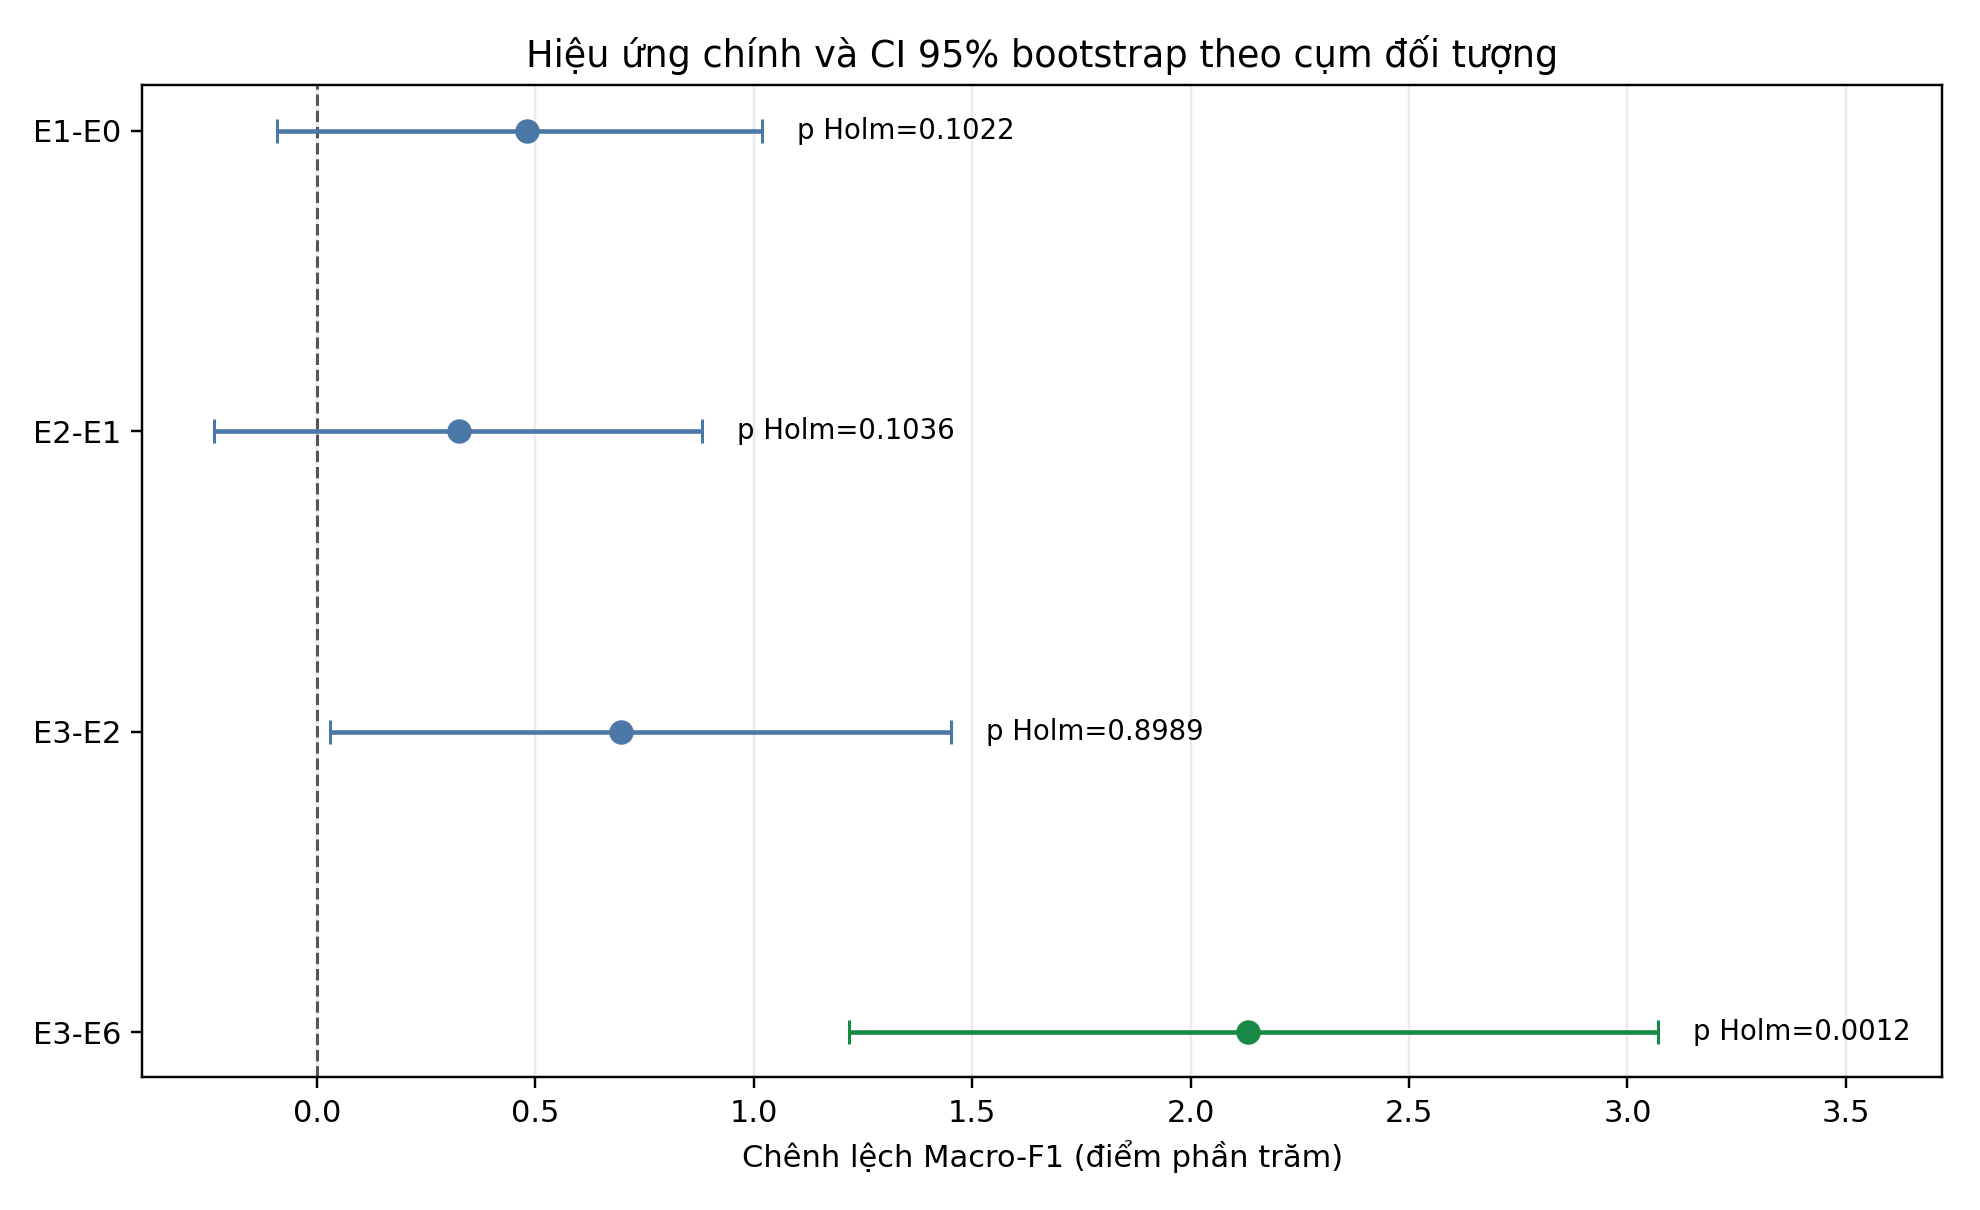
\includegraphics[width=\textwidth]{figures/gate8_primary_effects.png}
\caption{Chênh lệch \mf\ và khoảng tin cậy bootstrap cụm theo đối tượng. Trục hoành dùng điểm phần trăm.}
\label{fig:primary_effects}
\end{figure}

E1--E0 và E2--E1 có mức tăng mô tả nhỏ, nhưng CI chứa 0 và $p$ Holm lớn hơn 0,05. Vì vậy chưa đủ bằng chứng rằng TCN tốt hơn BiLSTM hoặc ResNet-1D tốt hơn 15CNN về \mf. E3--E2 có CI gộp vừa dương nhưng chỉ 37/78 người tăng, median chênh lệch theo người âm và Wilcoxon không có ý nghĩa; lợi ích không đồng đều theo đối tượng. E3--E6 là kết quả nhất quán nhất theo cả bootstrap và Wilcoxon-Holm.

\begin{table}[H]
\centering
\caption{Đối chiếu hậu nghiệm toàn pipeline E3 với mốc E0}
\label{tab:posthoc_e3_e0}
\begin{tabular}{lrrrr}
\toprule
\textbf{So sánh} & \textbf{$\Delta$ \mf} & \textbf{CI 95\% bootstrap} & \textbf{$p$ Wilcoxon} & \textbf{Thắng/Hòa/Thua} \\
\midrule
E3--E0 & 0,015024 & $[0,005746;\ 0,025871]$ & 0,012321 & 49/0/29 \\
\bottomrule
\end{tabular}
\end{table}

Đây là phân tích \emph{hậu nghiệm}, không thuộc bốn đối chiếu xác nhận ở Bảng~\ref{tab:primary_stats}. Nếu chỉ tham khảo phép Holm khi ghép nó thành so sánh thứ năm với bốn so sánh cũ, $p$ hiệu chỉnh là 0,049282; con số này không biến giả thuyết hậu nghiệm thành giả thuyết định trước. Kết quả hỗ trợ rằng toàn bộ pipeline E3 cao hơn E0 trong chiến dịch seed 42 hiện tại. Vì E3 và E0 đồng thời khác mô hình chuỗi, bộ trích xuất và tiền xử lý, đối chiếu này không xác định thành phần nào gây ra chênh lệch, không chứng minh ưu thế trên quần thể khác và không phải kiểm định tương đương hoặc không thua kém.

Chênh lệch F1 E3--E6 theo lớp lần lượt là W $+0,00255$, N1 $+0,01520$, N2 $+0,01295$, N3 $+0,06278$ và REM $+0,01311$. E4--E2, phân tích thứ cấp riêng lọc dải, có $\Delta=0,005586$, CI $[-0,001699;0,013618]$, $p=0,902877$ và thắng/thua 38/40; chưa có bằng chứng về cải thiện đồng đều.

\subsection{Gate 6: độ phức tạp và tốc độ}

\begin{table}[H]
\centering
\caption{Benchmark forward trên Tesla V100, 100 epoch mỗi lượt}
\label{tab:complexity}
\resizebox{\textwidth}{!}{%
\begin{tabular}{lrrrrrr}
\toprule
\textbf{E} & \textbf{Tham số} & \textbf{Độ trễ trung vị (ms)} & \textbf{p95 (ms)} & \textbf{Epoch/s} & \textbf{Peak MiB} & \textbf{Nhanh hơn E0} \\
\midrule
E0 & 248.630 & 13,4315 & 15,4400 & 7.445 & 58,81 & 1,00$\times$ \\
E1 & 640.950 & 12,5111 & 13,6892 & 7.993 & 60,31 & 1,07$\times$ \\
E2 & 1.085.578 & 3,5750 & 3,6531 & 27.972 & 75,54 & 3,76$\times$ \\
E3 & 1.085.578 & 3,5687 & 3,6813 & 28.021 & 75,54 & 3,76$\times$ \\
E4 & 1.085.578 & 3,5739 & 3,6427 & 27.980 & 75,54 & 3,76$\times$ \\
E6 & 1.085.578 & 3,5756 & 3,6426 & 27.967 & 75,54 & 3,76$\times$ \\
\bottomrule
\end{tabular}}
\end{table}

\begin{figure}[H]
\centering
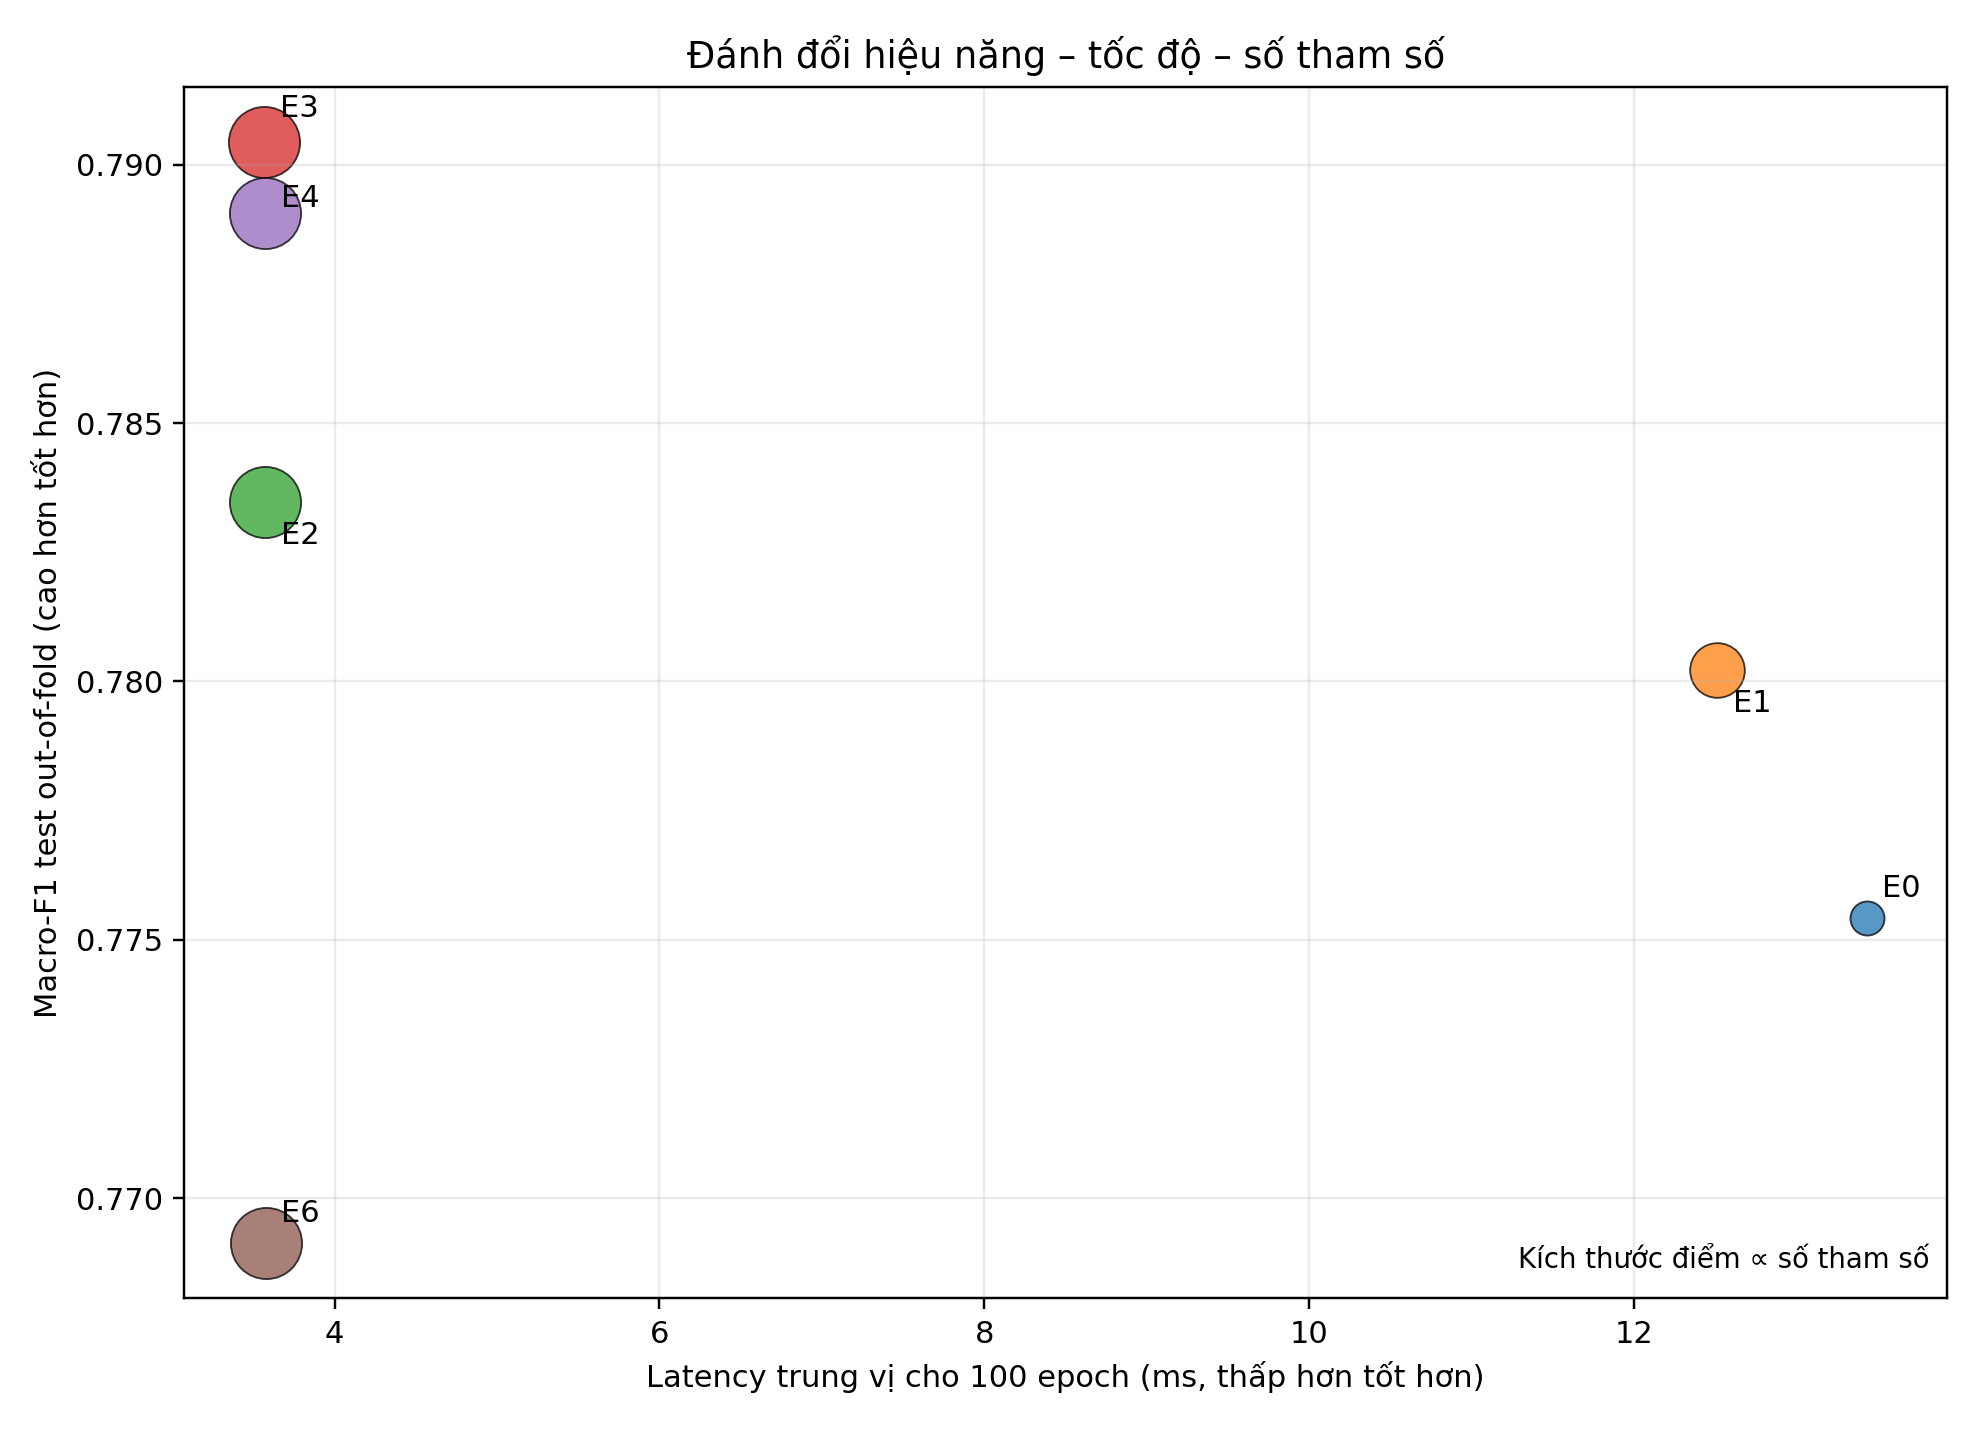
\includegraphics[width=0.9\textwidth]{figures/gate8_performance_speed_tradeoff.png}
\caption{Đánh đổi giữa \mf, độ trễ và số tham số. Diện tích điểm tỷ lệ với số tham số.}
\label{fig:tradeoff}
\end{figure}

ResNet-1D--TCN giảm từ 16 xuống 2 mô hình thành phần và nhanh hơn E0 khoảng 3,76 lần. Đổi lại, số tham số tăng 4,37 lần và peak VRAM tăng 28,4\%. Vì vậy kết quả hỗ trợ ``gọn hơn về vận hành'', không hỗ trợ ``mô hình nhẹ'' hoặc ``tiết kiệm tham số''.

\subsection{Gate 6: không gian đặc trưng}

Silhouette E2 thấp hơn E1 trong 10/10 fold. Chênh lệch E2--E1 trung bình là $-0,107851$, trung vị $-0,110025$ và khoảng quan sát $[-0,152622;-0,060811]$.

\begin{figure}[H]
\centering
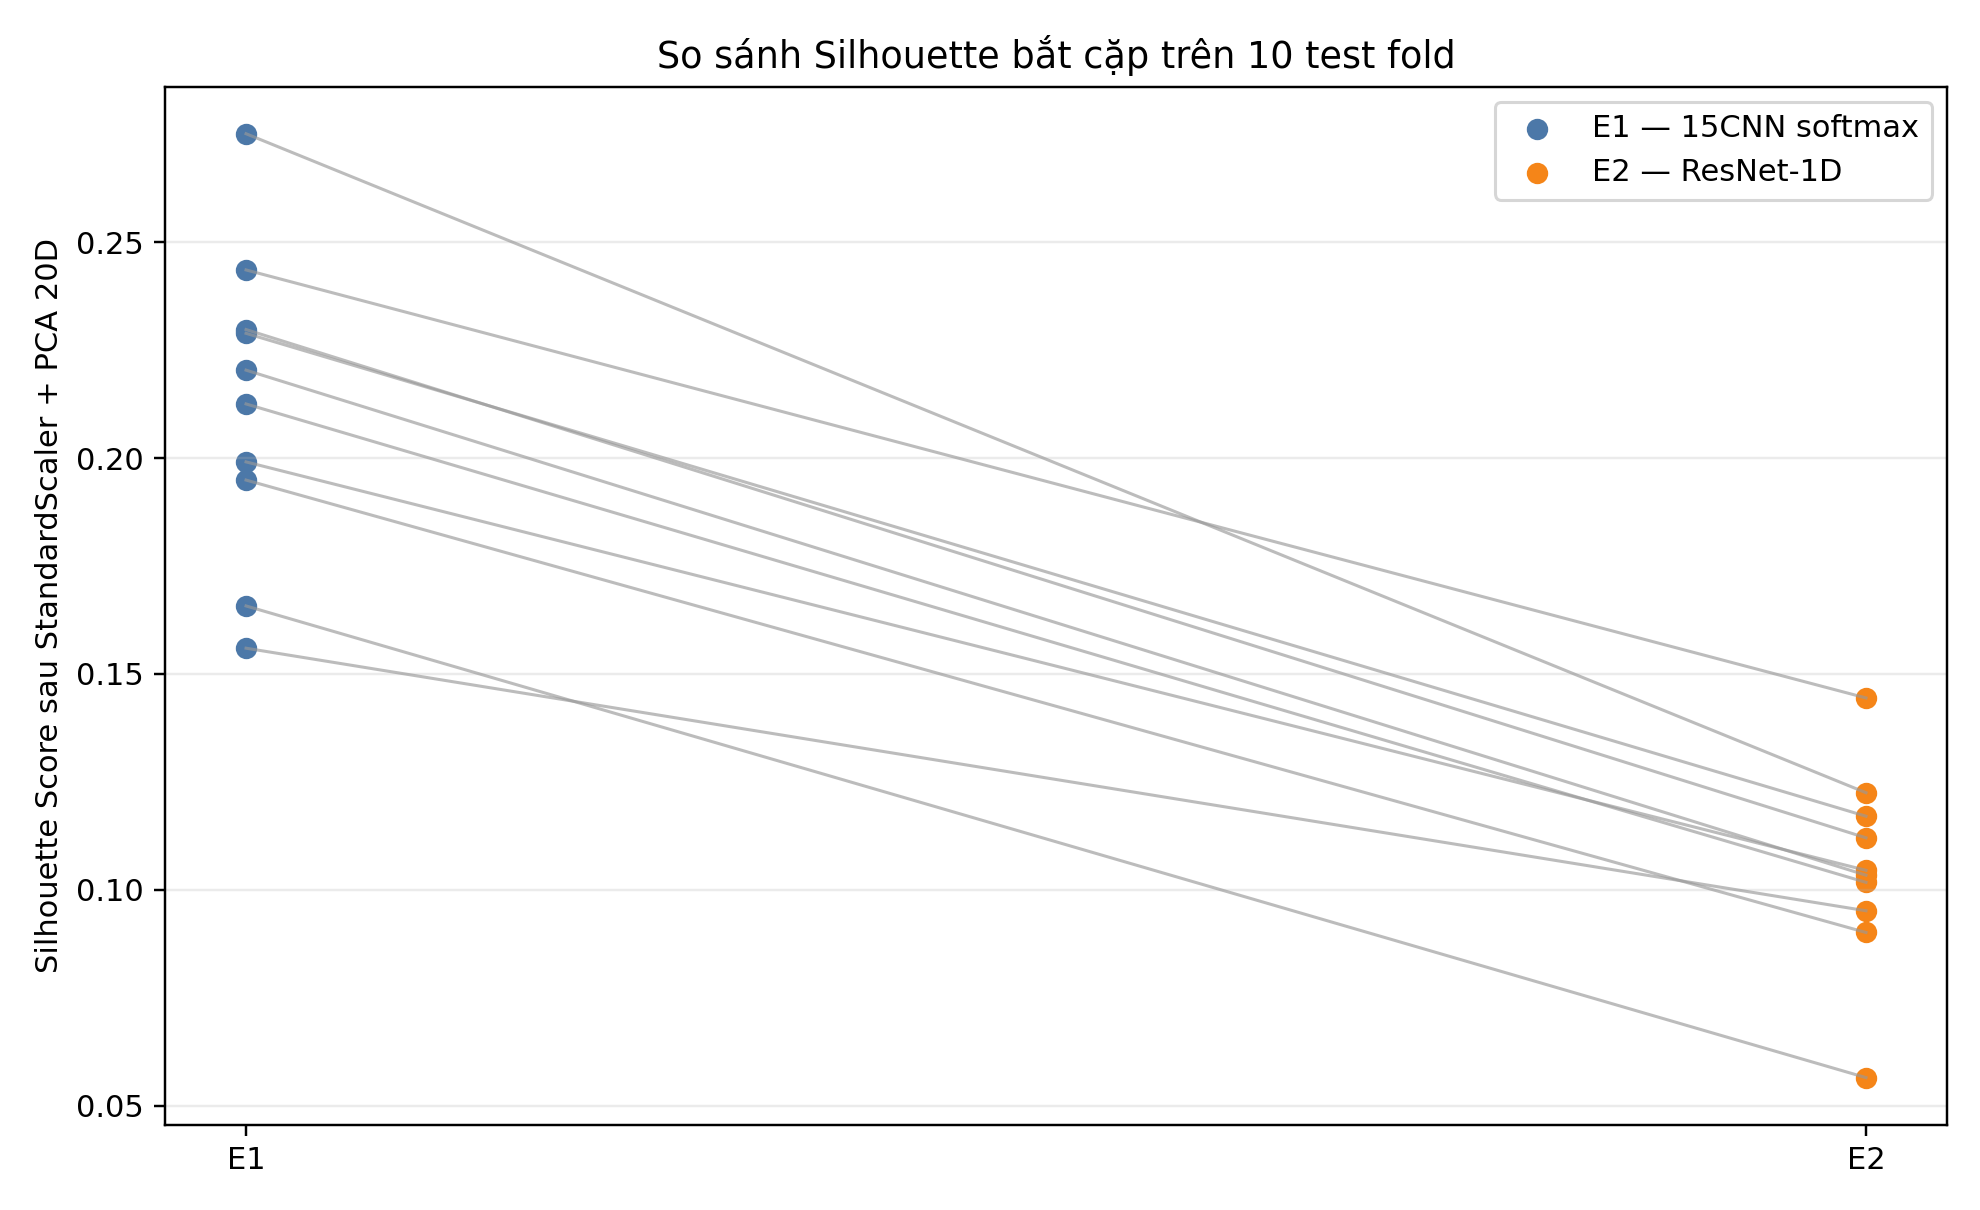
\includegraphics[width=\textwidth]{figures/gate8_feature_silhouette.png}
\caption{Silhouette bắt cặp E1/E2 sau StandardScaler và PCA 20 chiều.}
\label{fig:silhouette}
\end{figure}

Phép đo này không hỗ trợ giả thuyết rằng embedding ResNet có cụm Euclid tách biệt hơn softmax 15CNN. Nó cũng không chứng minh 15CNN tốt hơn cho dự đoán chuỗi, vì TCN có thể khai thác thông tin không biểu hiện dưới dạng cụm compact.

\subsection{Gate 7: gói công bố và truy nguyên}

Gate 7 không huấn luyện hoặc mở lại test. Cổng này sinh bảng CSV, hình, bản thảo tiếng Việt, ma trận tuyên bố--bằng chứng, manifest SHA-256 và trình kiểm định độc lập từ artifact Gate 5--6. Việc tách dữ liệu máy đọc khỏi văn bản giúp ngăn chép sai số và cho phép xây lại gói công bố.

\subsection{Gate 8: ablation nhóm C/P/N}

Gate 8 hoàn tất 30/30 lần huấn luyện validation và 30/30 lần suy luận test cho C, CP và CN; Full CPN tái sử dụng E1. Mỗi điều kiện phủ 78 đối tượng, 153 bản ghi và 195.469 epoch hợp lệ.

\begin{table}[H]
\centering
\caption{Kết quả mô tả ablation C/P/N}
\label{tab:gate8_descriptive}
\resizebox{\textwidth}{!}{%
\begin{tabular}{lrrrrr}
\toprule
\textbf{Điều kiện} & \textbf{\mf\ toàn bộ} & \textbf{F1 N1} & \textbf{Recall N1} & \textbf{\mf\ chuyển pha} & \textbf{Recall N1 chuyển pha} \\
\midrule
Full CPN & 0,780230 & 0,511469 & 0,503531 & 0,620055 & 0,483989 \\
C & 0,777477 & 0,501071 & 0,499907 & 0,619102 & 0,480828 \\
CP & 0,777733 & 0,502185 & 0,499257 & 0,617686 & 0,480163 \\
CN & 0,781585 & 0,505505 & 0,493867 & 0,618895 & 0,472428 \\
\bottomrule
\end{tabular}}
\end{table}

\begin{table}[H]
\centering
\caption{So sánh chính tại vùng chuyển pha $\pm1$ epoch}
\label{tab:gate8_stats}
\begin{tabular}{lrrrl}
\toprule
\textbf{So sánh} & \textbf{$\Delta$ \mf} & \textbf{CI 95\%} & \textbf{$p$ Holm} & \textbf{Thắng/Hòa/Thua} \\
\midrule
Full CPN--C & 0,000953 & $[-0,004588;0,006568]$ & 1,000 & 36/0/42 \\
Full CPN--CP & 0,002369 & $[-0,002990;0,007714]$ & 1,000 & 41/0/37 \\
Full CPN--CN & 0,001160 & $[-0,003918;0,006490]$ & 1,000 & 38/0/40 \\
\bottomrule
\end{tabular}
\end{table}

\begin{figure}[H]
\centering
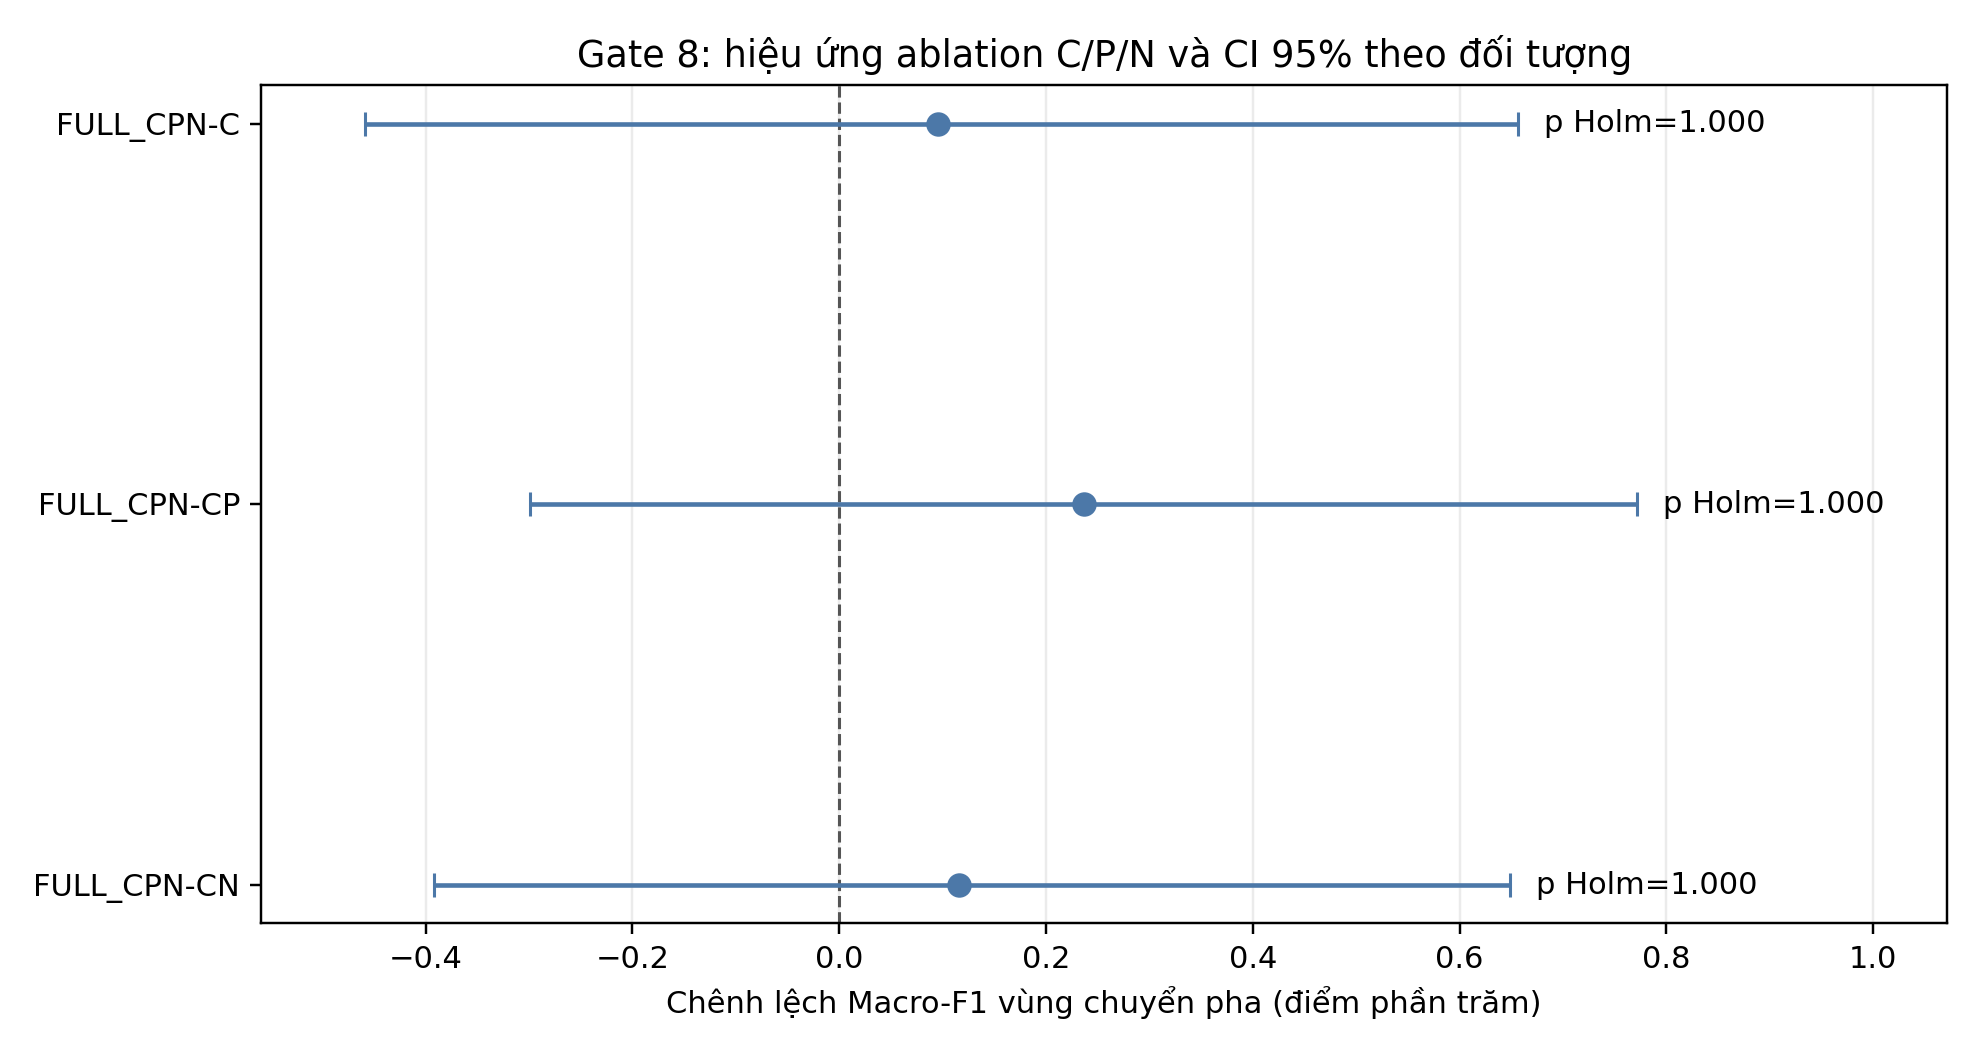
\includegraphics[width=\textwidth]{figures/gate8_context_ablation_effects.png}
\caption{Hiệu ứng ablation C/P/N tại vùng chuyển pha và CI bootstrap theo đối tượng.}
\label{fig:gate8_effects}
\end{figure}

Cả ba CI chứa 0, $p$ Holm đều bằng 1 và số người thắng/thua không nhất quán. Do đó chưa quan sát thấy lợi ích tăng thêm có ý nghĩa của P/N cho \mf\ vùng chuyển pha trong thiết kế hiện tại. Kết quả không chứng minh P/N vô dụng, không đo phần trăm thông tin và không thiết lập tương đương giữa các điều kiện.

\subsection{Chiến dịch SHHS1 zero-shot}

Tiền xử lý và hai cổng suy luận SHHS được thực hiện sau khi Gate 8 đã đóng. Validation gồm 15 đối tượng, 450 dự đoán theo fold và 45 tổ hợp; test gồm 180 đối tượng, 5.400 dự đoán theo fold và 540 tổ hợp. Hai cổng độc lập đều trả \code{PASSED} với 0 lỗi. Test có 169.012 epoch hợp lệ và mất 6.692,6 giây trên CPU 12 luồng.

\begin{table}[H]
\centering
\caption{Hiệu năng zero-shot trên 180 đối tượng SHHS1 đã khóa}
\label{tab:shhs_descriptive}
\resizebox{\textwidth}{!}{%
\begin{tabular}{lrrrrrr}
\toprule
\textbf{E} & \textbf{\mf\ đối tượng} & \textbf{CI 95\%} & \textbf{\mf\ gộp} & \textbf{Accuracy} & \textbf{$\kappa$} & \textbf{F1 N1} \\
\midrule
E0 & 0,5268 & $[0,5101;0,5431]$ & 0,5761 & 0,6648 & 0,5339 & 0,2998 \\
E3 & \textbf{0,5680} & $\mathbf{[0,5503;0,5850]}$ & \textbf{0,6099} & \textbf{0,7016} & \textbf{0,5801} & \textbf{0,3451} \\
E6 & 0,5407 & $[0,5227;0,5584]$ & 0,5732 & 0,6742 & 0,5408 & 0,3102 \\
\bottomrule
\end{tabular}}
\end{table}

\mf\ đối tượng là trung bình của 180 \mf\ tính riêng từng người và là tiêu chí chính. \mf\ gộp cho trọng số lớn hơn đối tượng có nhiều epoch nên chỉ là mô tả thứ cấp. E3 có giá trị cao nhất theo cả hai cách tổng hợp, accuracy, $\kappa$ và F1 N1.

\begin{table}[H]
\centering
\caption{Hai so sánh zero-shot chính bắt cặp theo đối tượng}
\label{tab:shhs_primary}
\resizebox{\textwidth}{!}{%
\begin{tabular}{lrrrrr}
\toprule
\textbf{So sánh} & \textbf{$\Delta$ \mf\ đối tượng} & \textbf{CI 95\%} & \textbf{Trung vị $\Delta$} & \textbf{Thắng/Hòa/Thua} & \textbf{$p$ Holm} \\
\midrule
E3--E0 & \textbf{0,0412} & $\mathbf{[0,0314;0,0512]}$ & 0,0372 & 138/0/42 & $2,65\times10^{-13}$ \\
E3--E6 & \textbf{0,0274} & $\mathbf{[0,0182;0,0370]}$ & 0,0292 & 125/0/55 & $1,87\times10^{-8}$ \\
\bottomrule
\end{tabular}}
\end{table}

\begin{figure}[H]
\centering
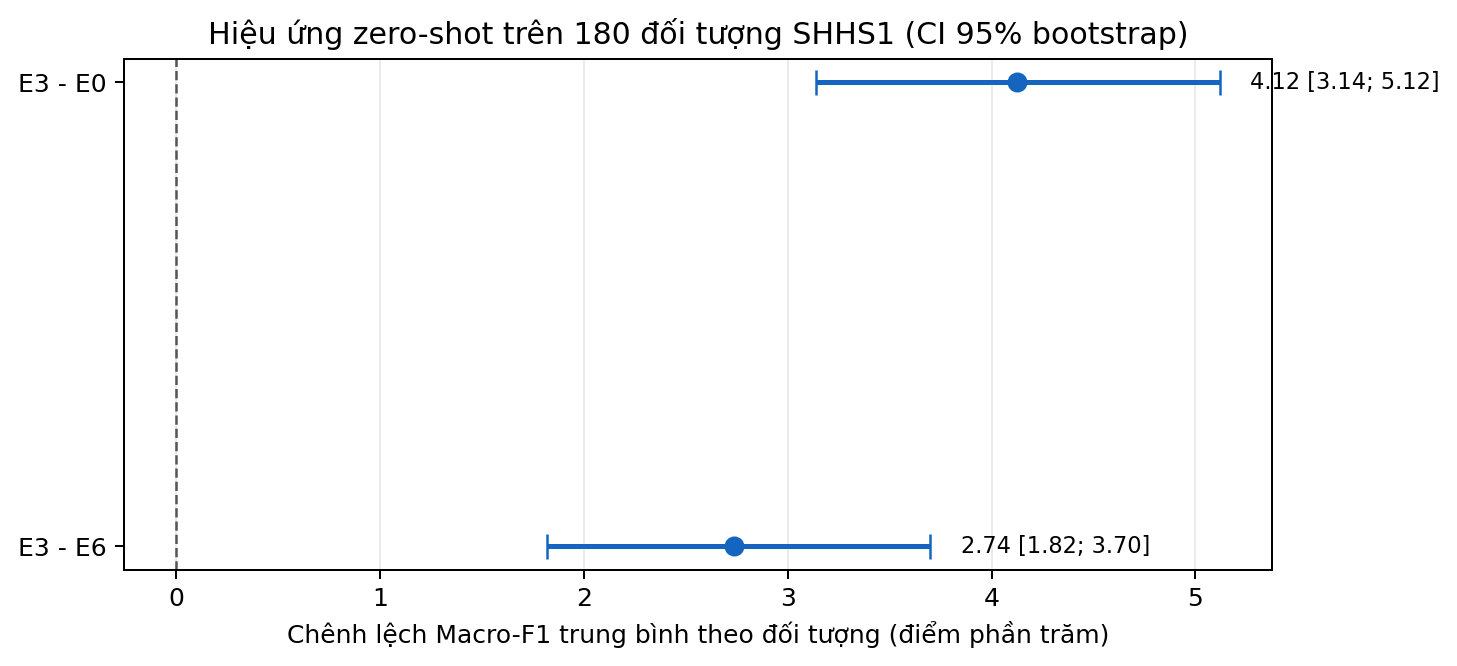
\includegraphics[width=0.92\textwidth]{figures/shhs_zero_shot_effects.png}
\caption{Chênh lệch \mf\ trung bình theo đối tượng và CI 95\% bootstrap cụm trên mẫu SHHS1. Đơn vị trục hoành là điểm phần trăm.}
\label{fig:shhs_effects}
\end{figure}

Cả hai CI chính hoàn toàn dương và Wilcoxon vẫn có ý nghĩa sau Holm. Do đó E3 có \mf\ trung bình theo đối tượng cao hơn E0 và E6 trong mẫu SHHS1 và giao thức zero-shot đã khóa. Các chỉ số hỗ trợ nhất quán: E3--E0 tăng \mf\ gộp 0,0338, accuracy 0,0368 và $\kappa$ 0,0461; E3--E6 tăng lần lượt 0,0367, 0,0274 và 0,0392. Tại 44.744 epoch nằm trong $\pm1$ epoch quanh chuyển pha thật liên tiếp, E3 tăng \mf\ so với E0 0,0366, CI $[0,0262;0,0471]$, và so với E6 0,0183, CI $[0,0092;0,0268]$.

N1 vẫn là lớp khó nhất. E3 có F1 N1 cao hơn E0/E6, nhưng recall N1 của E0 là 0,5841, cao hơn E3 0,5437; precision N1 của E3 là 0,2528, cao hơn E0 0,2017. Vì vậy lợi ích F1 của E3 phản ánh cân bằng precision--recall tốt hơn, không phải tăng đồng thời mọi chỉ số N1.

\subsection{Phân tích bổ sung thành phần E1/E2 trên SHHS1}

Sau chiến dịch zero-shot v1, một giao thức riêng được khóa trước lần suy luận SHHS đầu tiên của E1/E2. E0 được tái sử dụng nguyên trạng từ v1; E1 và E2 cùng dùng \code{paper\_raw\_v1}, đủ 10 checkpoint theo fold và không cập nhật trọng số bằng SHHS. Validation kỹ thuật gồm 300 dự đoán fold và 30 ensemble; test gồm 3.600 dự đoán fold và 360 ensemble. Hai cổng đều \code{PASSED} với 0 lỗi. Test dùng 180 đối tượng, 169.012 epoch và mất 5.681,1 giây trên CPU 12 luồng.

\begin{table}[H]
\centering
\caption{Hiệu năng mô tả trong phân tích thành phần SHHS1}
\label{tab:shhs_component_descriptive}
\resizebox{\textwidth}{!}{%
\begin{tabular}{lrrrrrr}
\toprule
\textbf{E} & \textbf{\mf\ đối tượng} & \textbf{\mf\ gộp} & \textbf{Accuracy} & \textbf{$\kappa$} & \textbf{F1 N1} & \textbf{\mf\ chuyển pha} \\
\midrule
E0 & 0,5268 & 0,5761 & 0,6648 & 0,5339 & 0,2998 & 0,4323 \\
E1 & \textbf{0,5333} & \textbf{0,5822} & \textbf{0,6709} & \textbf{0,5409} & \textbf{0,3197} & \textbf{0,4352} \\
E2 & 0,5205 & 0,5668 & 0,6656 & 0,5327 & 0,2833 & 0,4219 \\
\bottomrule
\end{tabular}}
\end{table}

\begin{table}[H]
\centering
\caption{So sánh bắt cặp trong phân tích thành phần SHHS1}
\label{tab:shhs_component_comparisons}
\resizebox{\textwidth}{!}{%
\begin{tabular}{lrrrrrl}
\toprule
\textbf{So sánh} & \textbf{$\Delta$ \mf\ đối tượng} & \textbf{CI 95\%} & \textbf{Trung vị $\Delta$} & \textbf{Thắng/Hòa/Thua} & \textbf{$p$ Holm} & \textbf{Quy tắc khóa trước} \\
\midrule
E1--E0 & \textbf{0,00651} & $\mathbf{[0,00192;0,01087]}$ & 0,00648 & 108/0/72 & 0,00325 & Đạt \\
E2--E1 & \textbf{$-0,01280$} & $\mathbf{[-0,02209;-0,00350]}$ & $-0,00429$ & 80/0/100 & 0,01005 & Không đạt \\
\bottomrule
\end{tabular}}
\end{table}

E1--E0 thỏa đồng thời điều kiện CI chính hoàn toàn dương và Wilcoxon có ý nghĩa sau Holm. Hiệu ứng nhỏ và lợi ích tại vùng chuyển pha chưa chắc chắn: $\Delta=0,00288$, CI $[-0,00297;0,00850]$. Giả thuyết E2 cao hơn E1 không đạt; chênh lệch quan sát có hướng ngược lại và cũng âm ở \mf\ gộp lẫn vùng chuyển pha. Vì 180 đối tượng này đã được mở trước cho E0/E3/E6, phân tích được mô tả là bằng chứng ngoại miền thứ cấp khóa trước suy luận E1/E2, không phải tái lập độc lập trên cohort chưa mở.

\subsection{Đối chiếu hậu nghiệm E3--E2 trên SHHS1}

E2 và E3 cùng dùng ResNet-1D--TCN nhưng khác chế độ dữ liệu: E2 dùng \code{paper\_raw\_v1}, còn E3 dùng \code{filtered\_v2}. Mọi dự đoán được ghép đúng 180 đối tượng và 169.012 epoch trước khi tính hiệu ứng.

\begin{table}[H]
\centering
\caption{Phân tích bắt cặp hậu nghiệm E3--E2 trên SHHS1}
\label{tab:shhs_e3_e2}
\resizebox{\textwidth}{!}{%
\begin{tabular}{lrrr}
\toprule
\textbf{Chỉ số E3--E2} & \textbf{Chênh lệch} & \textbf{CI 95\%} & \textbf{Ghi chú} \\
\midrule
\mf\ trung bình theo đối tượng & \textbf{0,04750} & $\mathbf{[0,03724;0,05792]}$ & Wilcoxon $p=2,35\times10^{-17}$ \\
\mf\ gộp & 0,04304 & $[0,03249;0,05364]$ & 169.012 epoch \\
Accuracy & 0,03599 & $[0,02542;0,04700]$ & Chỉ số hỗ trợ \\
$\kappa$ & 0,04737 & $[0,03382;0,06119]$ & Chỉ số hỗ trợ \\
F1 N1 & 0,06183 & $[0,03808;0,08572]$ & Chỉ số hỗ trợ \\
Recall N1 & 0,19095 & $[0,15125;0,22966]$ & Chỉ số hỗ trợ \\
\mf\ chuyển pha & 0,04700 & $[0,03790;0,05661]$ & Vùng $\pm1$ epoch \\
\bottomrule
\end{tabular}}
\end{table}

Trung vị chênh lệch \mf\ theo người là 0,04194 và E3 thắng/hòa/thua E2 trên 147/0/33 đối tượng. Tất cả CI hỗ trợ trong Bảng~\ref{tab:shhs_e3_e2} đều hoàn toàn dương. Vì vậy có bằng chứng hỗ trợ mạnh rằng toàn pipeline E3 tổng quát zero-shot tốt hơn E2 trên mẫu SHHS1 này. Trái lại, E3--E2 trên Sleep-EDF chỉ tăng \mf\ gộp 0,00696 nhưng Wilcoxon $p=0,89893$ và thắng/thua 37/41. Mẫu hình kết hợp phù hợp với cách diễn giải rằng lợi ích của chế độ tiền xử lý E3 biểu hiện rõ hơn khi chuyển miền; nó không chứng minh cơ chế nhân quả của từng thao tác tiền xử lý.
